\documentclass{beamer}
\usepackage[utf8x]{inputenc}
\usepackage[russian]{babel}
\usepackage{amsmath,mathrsfs,mathtext}
\usepackage{graphicx, epsfig}
\usetheme{Warsaw}%{Singapore}%{Warsaw}%{Warsaw}%{Darmstadt}
\usecolortheme{sidebartab}
\definecolor{beamer@blendedblue}{RGB}{15,120,80}
%----------------------------------------------------------------------------------------------------------
\title[\hbox to 56mm{Прогнозирование намерений  \hfill\insertframenumber\,/\,\inserttotalframenumber}]
{Декодирование сигналов мозга \\ и прогнозирование намерений}
\author[Д.\,С. Теленков]{\large \\Теленков Дмитрий Сергеевич}
\institute{\large
Московский физико-технический институт\par
Сколковский институт науки и технологий}

\date{\footnotesize{\emph{Курс:} Численные методы обучения по прецедентам\par (практика, В.\,В. Стрижов)/Группа 694, весна 2019}}
%----------------------------------------------------------------------------------------------------------
\begin{document}
%----------------------------------------------------------------------------------------------------------
\begin{frame}
%\thispagestyle{empty}
\titlepage
\end{frame}
%-----------------------------------------------------------------------------------------------------
\begin{frame}{Цель исследования}
\begin{block}{Цель работы}
Создать алгоритм выбора признаков, альтернативный PLS и учитывающий неортогональную структуру взаимозависимости признаков.
\end{block}
\begin{block}{Проблема}
Требуется научиться бороться с мультиколлинеарностью признаков
\end{block}
\begin{block}{Метод решения}
Использовать алгоритм иерархической смеси экспертов над моделью PLS
\end{block}
\end{frame}
%----------------------------------------------------------------------------------------------------------
\begin{frame}{Постановка задачи. Получение данных}
\begin{figure}[h!]
    \begin{minipage}[h!]{\linewidth}
    {\includegraphics[width=1\textwidth]{ArticleItself/Palm.png}} \\
    \end{minipage}
\label{fg:Example}
\end{figure}
\end{frame}
%----------------------------------------------------------------------------------------------------------
\begin{frame}{Постановка задачи. Описание данных}
Дана выборка размера $m$:
$$D_n = \{x_i, y_i\}^m_{i=1}$$
где $x_i \in \mathbb{R}^n$ - вектор признаков, $y_i \in \mathbb{R}^5$. Будем также говорить, что у нас есть матрица параметров $X$ и матрица ответов $Y$ \par
Выборка разбита на обучение и контроль:
$$D_\tau = \{x_i, y_i\}_{i\in\tau}\ \ D_\theta = \{x_i, y_i\}_{i\in\theta}\ \ \tau \sqcup \theta = [1, 2, \ldots, m]$$
Требуется научиться предсказывать значения $y_i$ по $x_i$ на обучении и проверить точность на контроле
\end{frame}
%----------------------------------------------------------------------------------------------------------
\begin{frame}{Список литературы}
[1] Schalk, G., Kubanek, J., Miller, K.J., Anderson, N.R., Leuthardt, E.C., Ojemann, J.G., Limbrick, D., Moran, D.W., Gerhardt, L.A., and Wolpaw, J.R. Decoding TwoDimensional Movement Trajectories Using Electrocorticographic Signals in Humans, J Neural Eng, 4: 264-275, 2007. \par
[2] Decoding Ipsilateral Finger Movements from ECoG Signals in Humans \par
[3] J. Wolpaw, N. Birbaumer, D. McFarland, G. Pfurtscheller, and T. Vaughan. Brain-computer interfaces for communication and control. Clinical neurophysiology, 113(6):767–791, 2002. \par 
[4] G. Pfurtscheller, C. Guger, G. Muller, G. Krausz, and C. Neuper. Brain oscillations control hand orthosis in a tetraplegic. Neuroscience letters, 292(3):211–214, 2000. \par
[5] J. Wolpaw and D. McFarland. Control of a two-dimensional movement signal by a noninvasive brain-computer interface in humans. Proceedings of the National Academy of Sciences of the United States of America, 101(51):17849, 2004.
\end{frame}
%----------------------------------------------------------------------------------------------------------
\begin{frame}{Базовый алгоритм. PLS}
\begin{block}{Понижение размерности и корреляции}
Векторы признаков $x_i$ имеют высокую размерность и сильно коррелированы. Для улучшение ситуации используется метод partial least squares
\end{block}
\begin{block}{PLS}
Находит переход из пространства параметров $\mathbb{R}^n$ в пространство более низкой размерности - $\mathbb{R}^k,\ k < n$, основываясь на корреляции между параметрами и ответами. Таким образом у нас появляется матрица перехода - $W_{n \times k}$
\end{block}
\begin{block}{Новая задача}
Задача линейной регрессии переходит в нахождении $Q \in \mathbb{R}^k$, что:
$$Y = T Q + E = X W Q + E$$
\end{block}

\end{frame}
%----------------------------------------------------------------------------------------------------------
\begin{frame}{Базовый алгоритм. NIPALS}
Для решения задачи PLS используем алгоритм NIPALS:\\
$A_1 = X^TY,\ M_1 = X^TX,\ C_1 = I$.\\ На $i$-й итерации алгоритма происходит:
\begin{enumerate}
    \item вычислим $e_i$, доминантный собственный вектор $A_i^TA_i$
    \item $w_i = C_i A_i e_i$, $w_i = \frac{w_i}{||w_i||}$. Положим $w_i$ в $W$, как $i$-ю колону
    \item $p_i = M_i w_i,\ c_i = w_i^T M_i w_i,\ p_i = \frac{p_i}{c_i}$
    \item $q_i = \frac{A_i^T w_i}{c_i}$. Положим $q_i$ в $Q$, как $i$-ю колону
    \item $A_{i + 1} = A_i - c_i p_i q_i^T, M_{i + 1} = M_i - c_i p_i p^T_i$
    \item $C_{i + 1} = C_i - w_i p_i^T$
\end{enumerate}
 Чтобы перейти к размерности $k$ необходимо сделать $k$ итераций.
\end{frame}
%----------------------------------------------------------------------------------------------------------
\begin{frame}{Вычислительный эксперимент. Данные}
\begin{block}{Получение}
Датасет взят из схожей работы [1]. В нем показаниям с 64 каналов кортикограммы сопоставлялись натяжения во всех пяти пальцах руки испытуемой. Частота сэмплирования - 1кГц, полоса пропускания каналов - 0.15-200Гц.
\end{block}
\begin{block}{Датасет}
Датасет состоит из элементов:
$$D_n = \{x_i, y_i\}^{4\cdot10^6}_{i=1},$$
где $x_i \in \mathbb{R}^{64}$ - вектор признаков, $y_i \in \mathbb{R}^5$.\\
\end{block}
\end{frame}
%----------------------------------------------------------------------------------------------------------
\begin{frame}{Вычислительный эксперимент. Базовый алгоритм}
\begin{figure}[h]
    \begin{minipage}[h]{0.4\linewidth}
    \center{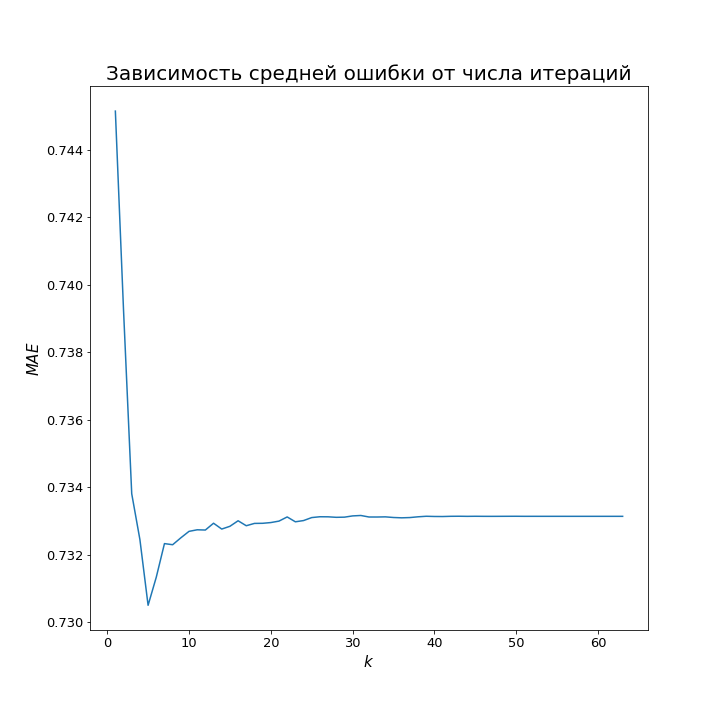
\includegraphics[width=1\textwidth]{ArticleItself/error.png}} \\
    \caption{Зависимость \\ средней ошибки от числа итераций.}
    \end{minipage}
    \hfill
    \begin{minipage}[h]{0.4\linewidth}
    \center{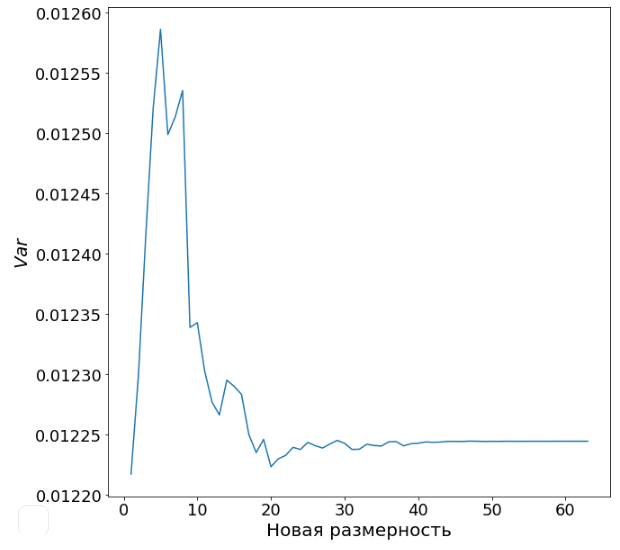
\includegraphics[width=1\textwidth]{ArticleItself/dispersion.png}} \\
    \caption{Зависимость дисперсии средней ошибки от числа итераций.}
    \end{minipage}
\label{fg:Example}
\end{figure}
\begin{block}{}
Минимум достигается при размерности пространства совпадающей с количеством пальцев. Но дисперсия ошибки там сильно возрастает.
\end{block}
\end{frame}
%----------------------------------------------------------------------------------------------------------
\begin{frame}{Вычислительный эксперимент. Базовый алгоритм}
\begin{figure}[h]
    \begin{minipage}[h]{0.4\linewidth}
    \center{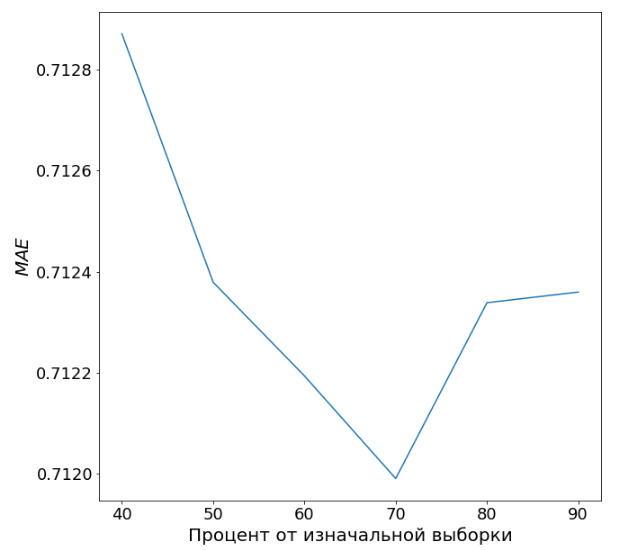
\includegraphics[width=1\textwidth]{ArticleItself/error_vol.png}} \\
    \caption{Зависимость средней ошибки от размера выборки.}
    \end{minipage}
    \hfill
    \begin{minipage}[h]{0.4\linewidth}
    \center{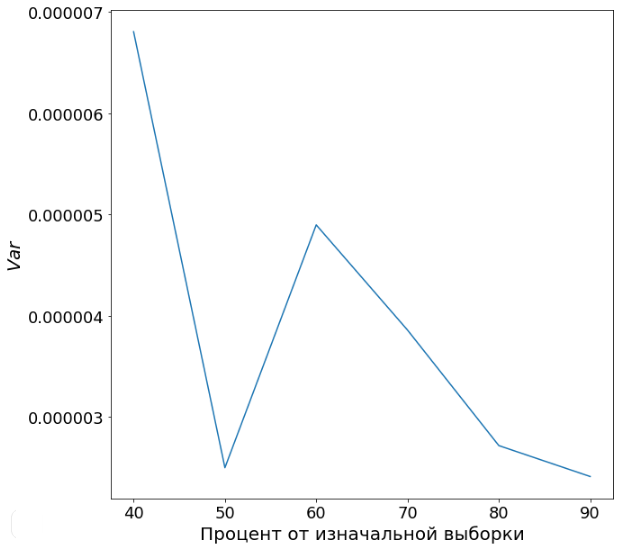
\includegraphics[width=1\textwidth]{ArticleItself/dispersion_vol.png}} \\
    \caption{Зависимость дисперсии средней ошибки от размера выборки.}
    \end{minipage}
\label{fg:Example}
\end{figure}
\begin{block}{}
Возможно переобучение при слишком большой выборке.
\end{block}
\end{frame}
%----------------------------------------------------------------------------------------------------------
\begin{frame}{Заключение}
Здесь мог бы быть мой основной алгоритм
\end{frame}
%----------------------------------------------------------------------------------------------------------
\end{document} 